\chapter{Grundlegende Konzepte}
\label{chap:grundlagen}

noch zu erkl�ren:
- benutzte Terminologie
- Modellgetriebene Software-Entwicklung
- Tests, Testdatengenerierung
- Literatur nutzen

\section{Modellgetriebene Software-Entwicklung}


\begin{itemize}
	\item \textbf{M0}: Konkrete Information
	\item \textbf{M1}: Meta-Daten zum Beschreiben der Information. Auch als \textit{Modell} bezeichnet.
	\item \textbf{M2}: 
	\item \textbf{M3}:
\end{itemize}

- Modell, Meta-Modell, Modell-Ebenen
- http://www.omg.org/spec/MOF/ISO/19502/PDF/ spricht von den klassischen 4 schichten...
- DSL, intern vs extern

\section{Software-Tests}
\label{sec:grundlagen:konzepte:tests}

\nomenclature{SUT}{System Under Test (\refsec{sec:grundlagen:konzepte:tests})}
Das zu testende System wird im Rahmen von Software-Tests als \textit{System Under Test} (abgek�rzt SUT) bezeichnet. Dabei kann
es sich je nach Test und Kontext auf Klassen, Objekte, Methoden, vollst�ndige Anwendungen oder Teile davon beziehen. 
\cite[810f]{XUNIT_TEST_PATTERNS}

Alle Voraussetzungen und Vorbedingungen f�r einen Testlauf werden unter der Bezeichnung \textit{Test Fixture} zusammengefasst.
Es repr�sentiert den Zustand des SUT vor den Tests. \cite[814]{XUNIT_TEST_PATTERNS} Es gibt verschiedene Arten von Test Fixtures.
Die im Rahmen dieser Arbeit relevanten sind \textit{Standard Fixture} und \textit{Minimal Fixture}.

Ein Test Fixture wird als Standard Fixture bezeichnet, wenn es f�r alle bzw. fast alle Tests verwendet werden kann. Ein Standard
Feature reduziert nicht nur den Aufwand zum Entwerfen von Testdaten f�r die einzelnen Tests, sondern verhindert dar�ber hinaus,
dass der Test-Ingenieur  sich bei verschiedenen Tests immer wieder in unterschiedliche Test-Daten hineinversetzen muss. Nur in
Ausnahmef�llen sollten Tests modifizierte oder eigene Testdaten verwenden. (\cite[305]{XUNIT_TEST_PATTERNS})

Minimal Fixtures stellen Test Fixtures dar, deren Umfang auf ein Minimum reduziert wurde. Dadurch lassen sich Minimal Fixtures
im Allgemeinen leichter verstehen. Das Reduzieren der Daten kann auch zu Leistungsvorteilen bei der Ausf�hrung der Tests f�hren.
(\cite[302]{XUNIT_TEST_PATTERNS})

%\subsection{Datenbanktests}
Eine �bliche Vorgehensweise, Systeme in Verbindung mit Datenbanken zu testen, stellt \textit{Back Door Manipulation} dar.
Dabei wird die Datenbank �ber direkten Zugriff, vorbei am zu testenden System, in den Anfangszustand gebracht.
Anschlie�end k�nnen die zu testenden Operationen am System durchgef�hrt werden. Um zu �berpr�fen, ob sich das System richtig
verhalten hat, wird der Zustand der Datenbank mit dem erwarteten Zustand verglichen - ebenfalls am zu testenden System vorbei.
\cite[327ff]{XUNIT_TEST_PATTERNS}

\todo{Grafik Back Door Manipulation}

Es gibt mehrere Vorteile, die Datenbank nicht �ber das zu testende System in den Anfangszustand zu bringen. Einerseits k�nnen
semantische Fehler im zu testenden System unter Umst�nden nur so gefunden werden. Andererseits kann der Zustand mitunter
schneller in die Datenbank geschrieben werden, wenn nicht der Weg �ber das zu testende System gemacht wird. Au�erdem bietet es
in Bezug auf die Zust�nde eine h�here Flexibilit�t: Die Datenbank kann auch in Zust�nde	gebracht werden, die �ber das System
nicht erreicht werden k�nnen. Daf�r leidet die Flexibilit�t an einer anderen Stelle: Die Tests sind abh�ngig vom konkret
verwendeten Datenbank-System. Au�erdem setzt der direkte Zugriff auf die Datenbank voraus, dass die Semantik der
zu testenden Anwendung ber�cksichtigt wird. Aus Sicht der Anwendung d�rfen sich von der Anwendung eingespielte Daten in ihrer
Form nicht von den manuell in die Datenbank geschriebenen Daten unterscheiden.


\todo{Layer test erkl�ren}

\section{Konventionen}
\label{sec:grundlagen:konventionen}

	\subsection{Datenbank-Diagramme}
	\label{sec:grundlagen:konventionen:datenbankdiagramme}
	F�r die Darstellung von Datenbank-Diagrammen wird ein einheitlicher Stil verwendet. Dieser orientiert sich an
	Ambler aus \cite{REFACTORING_DATABASES}. Auf die Angabe von Stereotypen wird sowohl bei den Tabellen, als auch
	bei den Beziehungen zwischen Tabellen verzichtet.
	
	Erkl�ren:
	- Spalten/PK/FK
	- Karidnalit�ten
	
	Abbildung \ref{img:ambler_table} zeigt ein Diagramm mit zwei Tabellen. Tabelle 2 enth�lt einen Fremdschl�ssel,
	der einem Prim�rschl�ssel aus Tabelle 1 

	\begin{figure}[H]
		\centering
		 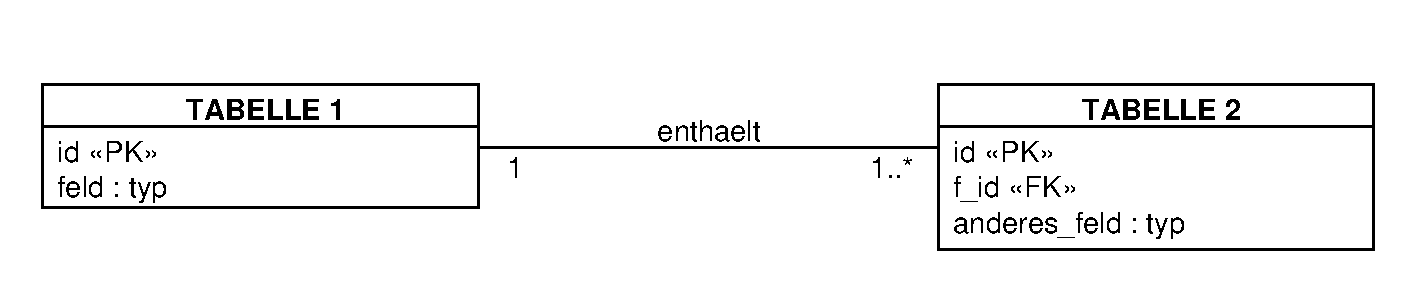
\includegraphics[width=0.75\textwidth]{images/grundlagen/ambler_table.pdf}
		\caption{Datenbank-Diagramm-Stil nach Ambler}\label{img:ambler_table}
	\end{figure}

